\documentclass[conference]{IEEEtran}
% Compiled with XeTeX (Tectonic), so Times comes from TeX Gyre Termes, an OpenType Times clone.
\usepackage{amsmath}
\usepackage{fontspec}
\setmainfont{texgyretermes}[Extension=.otf, UprightFont=*-regular, BoldFont=*-bold,
  ItalicFont=*-italic, BoldItalicFont=*-bolditalic]
\usepackage{unicode-math}
\setmathfont{texgyretermes-math.otf}
\usepackage{cite}
\usepackage{array}
\usepackage{booktabs}
\usepackage{url}
\usepackage{tikz}
\usetikzlibrary{arrows.meta}
\newcolumntype{L}[1]{>{\raggedright\arraybackslash}p{#1}}

\begin{document}

\title{FEAther: A Self-Learning Multi-Agent System for Lightweight Load-Bearing Part Design with Finite Element Analysis}

\author{\IEEEauthorblockN{Rifqi Wibisono}
\IEEEauthorblockA{Nanjing Xiaozhuang University, Nanjing, China\\
Student ID L25020014}}

\maketitle

\begin{abstract}
We propose to use reinforcement learning to train an open-weight large language model (LLM) to write
computer-aided design (CAD) programs for load-bearing parts, rewarded by a finite element analysis
(FEA) of the part each program produces. Current text-to-CAD models are trained and judged on whether a
shape resembles a reference; whether the part carries its load is never checked. FEAther is a
multi-agent system built around one trained agent. An untrained parser turns a request into a
structured specification; the trained designer writes a CadQuery program; a sandboxed checker runs it,
meshes the part, solves it with CalculiX, and returns a graded reward with a report. The system is
self-learning: the designer is trained on its own scored attempts, and at run time it revises its design
from the report until the part passes, then removes material while it still passes.
We ask whether an FEA-graded reward beats a shape-similarity reward (RQ1), whether run-time feedback adds
anything beyond training or only adds attempts (RQ2), and how much material the passing designs use
(RQ3). A pilot has built the oracle and the data. The checker's FEA agrees with hand calculations within
10\% on ten reference parts. Forty generated specifications are each proven solvable. The untrained
Qwen3-1.7B and Qwen3-8B models solve none of them, and repeat their own failed program in about 80\% of
revision attempts.
\end{abstract}

\begin{IEEEkeywords}
code generation, CAD, finite element analysis, reinforcement learning, self-repair, test oracle
\end{IEEEkeywords}

\section{Introduction}

% Defined here so that it floats to the top of page 2, next to Section III.
\begin{table*}[t]
\caption{Research questions, variables and analysis}
\label{tab:rq}
\centering\footnotesize
\begin{tabular}{@{}L{0.32\textwidth}L{0.25\textwidth}L{0.22\textwidth}L{0.13\textwidth}@{}}
\toprule
Question & Independent variable & Dependent variable & Analysis\\
\midrule
RQ1: Does GRPO with an FEA-graded reward raise the share of held-out specs fully passed, compared with
SFT alone and with a shape-similarity reward?
& training: SFT only; GRPO with a shape reward, an FEA reward, or both
& full pass rate; share of requirements met; invalid rate
& McNemar's test; bootstrap 95\% intervals\\
\addlinespace
RQ2: Does run-time FEA feedback improve designs beyond what training put into the model, and is the gain
from the feedback or from more attempts?
& designer: SFT, GRPO, GRPO with revise and lighten prompts; attempts: one-shot, best-of-$k$, loop;
$k\in\{1,3,5,10\}$
& specs passed within $k$; mass of the lightest pass; tokens per solved spec
& McNemar's test at each $k$\\
\addlinespace
RQ3: How much material do passing designs use, and what does the reward's mass term change?
& reward with or without the mass term
& mass relative to sizing-only and topology-optimised references; pass rate
& Wilcoxon signed-rank test\\
\bottomrule
\end{tabular}
\end{table*}

A parametric CAD model can be written as a program. In CadQuery~\cite{cadquery}, a Python library on the
OpenCASCADE geometry kernel, a bracket is a script that sketches profiles, extrudes them and cuts holes;
running it yields a solid that can be meshed, simulated and printed. Because such programs are text,
LLMs can learn to write them, and recent models translate text, images or point clouds into
CadQuery~\cite{rukhovich2024cadrecode,guan2025cadcoder,kolodiazhnyi2026cadrille}.

These models are trained and evaluated on geometric resemblance: a reward or metric compares the
generated shape with a reference shape, for example by Chamfer distance. For a load-bearing part,
resemblance is the wrong oracle. Two brackets that look alike can differ widely in peak stress, because
stress concentrates at small features such as the inside radius of a bend or the edge of a
hole~\cite{budynas2020shigley,pilkey2008peterson}. Regenwetter et al.\ showed that similarity metrics
miss engineering performance~\cite{regenwetter2023beyond}. When designs are checked by physics, current
systems fail: in Son et al.'s 50 FEA-checked engineering briefs, no frontier agent's first design passed
every requirement~\cite{son2026selfimproving}, and CADEngBench reports that matching a reference FEA
response ``remains difficult''~\cite{singh2026cadengbench}.

From a software-engineering view, a CAD program is code whose test oracle is physics. Code-generation
research offers two lessons that should transfer: execution feedback can train a model through
reinforcement learning, and feedback at run time (self-repair) helps less than expected once its extra
attempts are paid for~\cite{olausson2024selfrepair}. Neither has been tested with a physics oracle.

The closest work, COSMO-Agent~\cite{deng2026cosmo}, trains Qwen3-8B with the GRPO algorithm and the
CalculiX solver in the loop, but only to choose parameter values for 25 fixed CadQuery templates. In
engineering terms this is \emph{sizing}; it caps cost rather than minimising mass, and it used 16 H200
GPUs. No work we found trains a model to make \emph{configuration} choices (the layout: where material
goes, whether there is a rib or a cutout), written as a CAD program, against FEA-checked requirements.
Our last arXiv search, on 1~November 2026, found RL-trained CAD generators that still reward only shape
resemblance. This proposal contributes:
\begin{itemize}
\item an FEA test oracle for generated CAD programs, with sandboxed execution and a staged reward,
validated against hand calculations;
\item a specification generator in which every specification is proven solvable, and a sizing-only
baseline that separates configuration from sizing;
\item a recipe that trains one designer to design, revise and lighten on a single 16\,GB GPU;
\item an evaluation that separates the effect of feedback from the effect of more attempts.
\end{itemize}

\section{Related Work}

\textbf{LLMs that write CAD programs.} CAD-Recode reconstructs CadQuery programs from point clouds,
trained on one million procedurally generated programs~\cite{rukhovich2024cadrecode}. CAD-Coder
generates CadQuery from text, fine-tuned on about 110{,}000 text--code--shape triplets and then trained
with GRPO on a geometric reward~\cite{guan2025cadcoder}; cadrille applies reinforcement learning to
multi-modal reconstruction~\cite{kolodiazhnyi2026cadrille}. All of their rewards measure resemblance to
a target shape.

\textbf{Physics in the loop.} Son et al.\ give frontier agents FEA reports at run time and let them
iterate; their agents are called self-improving because they iterate on feedback, but no model is
trained~\cite{son2026selfimproving}. CADEngBench benchmarks parametric design against simulation
without training~\cite{singh2026cadengbench}. COSMO-Agent trains on simulation results but sizes fixed
templates~\cite{deng2026cosmo}. FEAther differs from all three by training the model that chooses the
configuration, and by rewarding low mass as well as passing.

\textbf{Self-repair in code generation.} Self-Debug~\cite{chen2024selfdebug} teaches models to fix their
code from execution results. Olausson et al.\ found that, at an equal budget, self-repair often gains
little over drawing more independent samples, because models rarely act well on
feedback~\cite{olausson2024selfrepair}. RQ2 tests this claim with a physics oracle, before and after
the repair skill is trained.

\section{Research Questions and Hypotheses}

Table~\ref{tab:rq} lists the questions, their variables and the planned analysis. The hypotheses are:
\textbf{H1:} the FEA-graded reward raises the full pass rate over both SFT alone and the shape reward,
because only it scores what a spec requires. \textbf{H2:} for untrained and SFT-only designers,
best-of-$k$ sampling matches or beats the loop at equal $k$, as in our pilot; after training on revise
and lighten prompts, the loop beats best-of-$k$. \textbf{H3:} without the mass term, passing designs are
no lighter than the sizing-only reference; with it, they are lighter, because the designer can move
material instead of only scaling it.

\section{Approach}

\begin{figure}[t]
\centering
\resizebox{\columnwidth}{!}{%
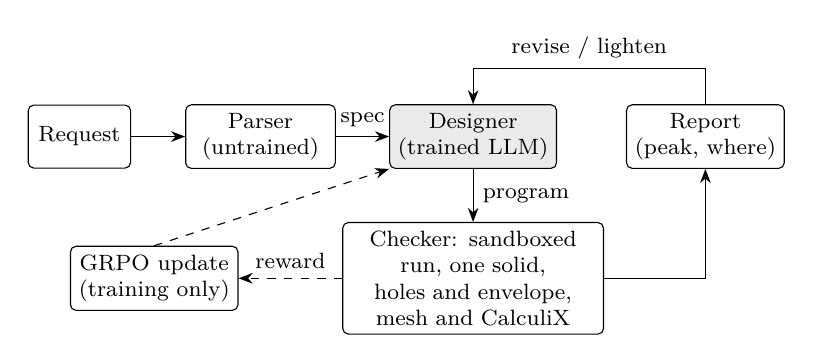
\begin{tikzpicture}[font=\footnotesize,
  box/.style={draw, rounded corners=2pt, align=center, inner sep=3pt, minimum height=8mm},
  arr/.style={-{Stealth[length=1.8mm]}}]
\node[box, minimum width=13mm] (spec) at (0,0) {Request};
\node[box, minimum width=19mm] (parse) at (2.3,0) {Parser\\(untrained)};
\node[box, minimum width=20mm, fill=black!8] (design) at (5.0,0) {Designer\\(trained LLM)};
\node[box, minimum width=17mm] (report) at (7.95,0) {Report\\(peak, where)};
\node[box, text width=31mm] (check) at (5.0,-1.8) {Checker: sandboxed run, one solid, holes and envelope, mesh and CalculiX};
\node[box, minimum width=19mm] (grpo) at (0.95,-1.8) {GRPO update\\(training only)};
\draw[arr] (spec) -- (parse);
\draw[arr] (parse) -- node[above]{spec} (design);
\draw[arr] (design) -- node[right]{program} (check);
\draw[arr] (check.east) -| (report.south);
\draw[arr] (report.north) -- ++(0,0.45) -| node[pos=0.25, above]{revise / lighten} (design.north);
\draw[arr, dashed] (check.west) -- node[above]{reward} (grpo.east);
\draw[arr, dashed] (grpo.north) -- (design.south west);
\end{tikzpicture}}
\caption{FEAther. Only the designer is trained; the parser and the report stay outside the reward
path. At run time the report drives revisions; in training the checker's reward updates the designer.}
\label{fig:system}
\end{figure}

\textbf{Specifications.} Each specification (spec) is a structured record and an English prompt that
states every number in it: a load (force, point, direction and patch radius), bolt holes (axis and
diameter), an envelope the part must stay inside, the material (PLA, Young's modulus 2300\,MPa) and
limits on peak stress, deflection and mass. A generator samples specs for each part family (first
L-brackets and wall hooks, about five by the end, with one or two families held out of training). It
sizes a reference program from that family's template by hand calculation and keeps the spec only if
the checker passes the reference. Each kept spec is therefore proven solvable. The reference then sets
two limits. The deflection limit is 1.3 to 2 times the reference's deflection. The mass budget is 80\%
of the reference's mass, because a budget at the reference would stop rewarding any design lighter than
what sizing alone achieves.

\textbf{Checker.} Programs from the model are untrusted. Each one runs in its own process with no
network (its own user and network namespaces) and with limits on memory, CPU time and file size; it
must leave its part in a variable named \texttt{result}. The checker then grades in stages, and credit
stops at the first that fails: the program runs (0.1); it makes exactly one valid solid (0.1); every
bolt hole is open where the spec puts it, a surface lies at the load point and the part stays in the
envelope (0.2); the structure (0.4, the mean over requirements of $\min(1,\text{limit}/\text{value})$
for peak stress and deflection); and the mass ($0.2\min(1,\text{budget}/\text{mass})$, counted only once
the structure passes). Gmsh~\cite{geuzaine2009gmsh} meshes the part with quadratic tetrahedra, refined
on curved faces, and CalculiX~\cite{dhondt2004fem} solves a linear static case: bolt bores held rigid,
the load spread over a patch. Both of these raise stress artificially near the bores and the patch, so
peak von Mises stress is read outside a zone one bolt diameter beyond each bore and twice the patch
radius round the load. The report states which stage failed, the peak stress, where it is and by how
much it misses its limit (Fig.~\ref{fig:example}).

\begin{figure}[t]
\centering\scriptsize
\fbox{\parbox{0.96\columnwidth}{\raggedright
\textbf{(a) Prompt of a generated spec.} I need a wall bracket that holds a load out from the wall,
printed in PLA. Stay within the box x 0 to 60, y -15 to 15, z -1 to 76 mm. Requirements: peak stress
under 10 MPa, deflection under 3.8 mm, and mass ideally below 9.3 g. Mount it on the wall at x = 0 with
2 M5 bolts; their 5.5 mm holes run along x at (y, z) = (0, 10) and (y, z) = (0, 43) mm. A 10 N load
presses straight down on it at the point (42, 0, 76) mm, spread over a patch of radius 4 mm.\\[3pt]
\textbf{(b) Checker report on reference part L1, built to fail.}\\
\texttt{FAIL at stage 'structure' (reward 0.70 of 1.00)}\\
\texttt{- Largest deflection 3.90 mm (no limit set).}\\
\texttt{- Peak stress 13.36 MPa at (6.6, 0.9, 61.4) mm;}\\
\texttt{\ \ limit 10.00 MPa, over the limit by 34\%.}\\
\texttt{- Mass 24.38 g (not scored until the structure passes).}}}
\caption{What the designer sees: (a) a spec's prompt, with every number in the spec; (b) the report it
revises from. The peak lies on the inside of L1's 2\,mm bend radius, where curved-beam theory puts it.}
\label{fig:example}
\end{figure}

\textbf{Agents and loop.} Fig.~\ref{fig:system} shows the system. The designer writes a program; while
it fails, the designer receives its own program and the report and revises; once it passes, it is asked
for a lighter version that still passes, and the lightest passing design is kept.

\textbf{Training.} The designer is Qwen3-8B~\cite{yang2025qwen3}, with Qwen3-1.7B for pilots.
Supervised fine-tuning (SFT) on public text-to-CadQuery data~\cite{guan2025cadcoder,rukhovich2024cadrecode}
teaches the language. Group Relative Policy Optimization (GRPO)~\cite{shao2024deepseekmath} then samples
a group of $G=8$ programs for each prompt, scores them with the checker ($r_1,\dots,r_G$) and gives each
program the advantage
\begin{equation}
A_i = \frac{r_i - \operatorname{mean}(r_1,\dots,r_G)}{\operatorname{std}(r_1,\dots,r_G)}.
\end{equation}
The update makes the tokens of programs with $A_i>0$ more likely and the rest less likely. A prompt whose
eight programs all score the same therefore teaches nothing, which is why the reward is graded rather
than pass/fail. Training mixes three prompt kinds, the same ones the loop uses: design; revise, with one
of the model's own failed programs and its report; and lighten, with a passing program.
QLoRA~\cite{dettmers2023qlora} freezes the base model in 4-bit precision and trains small adapter
matrices, which brings the 8B model within a 16\,GB laptop GPU (about 11\,GB, estimated). FEA rewards
run on 20 CPU workers at 2--7\,s each, so generating designs on the GPU is the bottleneck.

\section{Preliminary Results}

All results below come from the project repository and can be re-run with one command each.

\textbf{The oracle agrees with theory.} A cantilever beam gave a tip deflection of 1.736\,mm against
1.739\,mm from beam theory. Ten hand-written reference parts in three families put their worst point
where a reliable formula applies (Table~\ref{tab:oracle}): curved-beam theory for the bends of
L-brackets and hooks, and Heywood's formula for a hole in a strip~\cite{budynas2020shigley,pilkey2008peterson}.
On all ten, the checker's FEA peak lies within 10\% of the hand calculation and within 8\,mm of the
predicted point or its mirror image, and refining the mesh moves each value by under 4\%. The checker
fails the three parts built to exceed the 10\,MPa limit and passes the other seven, in 1.6--7.3\,s per
part. Separate tests confirm that a crashing program, an endless loop, a program grabbing 8\,GB, an
attempt to reach the network, a part in two pieces, a missing bolt hole and a hole 0.7\,mm too large
each fail at the right stage.

\begin{table}[t]
\caption{Checker FEA against hand calculations (peak stress)}
\label{tab:oracle}
\centering\footnotesize
\begin{tabular}{@{}lcll@{}}
\toprule
Family & Parts & Hand calculation at worst point & FEA / hand\\
\midrule
L-bracket & 4 & curved beam (Winkler), bend & 1.046--1.096\\
Wall hook & 3 & curved beam (Winkler), curve & 0.975--1.047\\
Hanger strap & 3 & hole in a strip (Heywood) & 1.013--1.024\\
\bottomrule
\end{tabular}
\end{table}

\textbf{Every spec is solvable.} The generator produced 40 specs, 20 L-brackets and 20 hooks, in 104\,s
on eight workers; every reference passed on its first FEA run, with peaks of 7.6--9.1\,MPa against the
10\,MPa limit.

\textbf{Untrained models solve nothing.} We served Qwen3-1.7B (16-bit) and Qwen3-8B (8-bit floating
point) with vLLM~\cite{kwon2023vllm}, thinking mode off, and gave each eight checker runs per spec,
either as eight independent samples or in the loop (Table~\ref{tab:baseline}). Neither model passed a
spec. Most programs misuse the CadQuery interface; those that make a solid cross into the wall, because
CadQuery centres boxes on the origin. In the loop, about 80\% of revisions (225 of 280 for 1.7B, 221 of
280 for 8B) repeat the program they were asked to fix, so independent samples reach running code on more
specs than the loop does (34 against 18 for the 8B). This agrees with Olausson et al.~\cite{olausson2024selfrepair}
and is the baseline that trained revision must beat. GRPO would already have a signal on 34 of 40 specs,
where the 8B's samples score differently, but only between the credits for running, for one solid and
for the interfaces; no design reached the structural checks. SFT therefore comes first.

\begin{table}[t]
\caption{Untrained baseline: specs (of 40) whose best of eight attempts got past each stage}
\label{tab:baseline}
\centering\footnotesize
\setlength{\tabcolsep}{4pt}
\begin{tabular}{@{}lcccc@{}}
\toprule
& \multicolumn{2}{c}{Qwen3-1.7B} & \multicolumn{2}{c}{Qwen3-8B}\\
\cmidrule(lr){2-3}\cmidrule(l){4-5}
Stage passed & samples & loop & samples & loop\\
\midrule
program runs & 8 & 1 & 34 & 18\\
one valid solid & 5 & 1 & 12 & 4\\
holes, envelope & 0 & 0 & 0 & 0\\
all requirements & 0 & 0 & 0 & 0\\
\bottomrule
\end{tabular}
\end{table}

\section{Evaluation Plan}

\textbf{Test material.} Held-out specs, including whole held-out families, and Son et al.'s briefs if
they are released~\cite{son2026selfimproving}.

\textbf{Baselines.} The untrained model; the SFT-only model; SFT plus GRPO with a shape-similarity
reward, as in CAD-Coder~\cite{guan2025cadcoder}; and a sizing-only search that tunes the reference
template's parameters without an LLM. The last isolates what choosing the configuration adds over
sizing, the difference from COSMO-Agent.

\textbf{Measures.} The full pass rate (share of specs meeting every requirement); the share of
requirements met; the invalid rate (programs that crash or make no single solid); mass relative to the
references; the pass rate within $k$ attempts; and tokens and seconds per solved spec.

\textbf{Statistics.} Every condition attempts the same specs, so pass/fail outcomes are paired and
compared with McNemar's test, which counts only the specs on which two conditions disagree. Rates carry
bootstrap 95\% intervals, and mass ratios use the Wilcoxon signed-rank test, which does not assume
normally distributed differences. As an extension, a subset of before-and-after designs will be
3D-printed and broken to compare measured failure loads with FEA.

\section{Threats to Validity}

\textit{Construct.} The oracle is a simplified model: linear static, rigid bolts, no contact, and an
isotropic material, while printed PLA is weaker across its layers. Validation against hand
calculations and the planned physical tests bound this. \textit{Internal.} A trained model may exploit
the oracle, for example with geometry that meshes oddly; the staged checks, the stress-reading zones,
mesh-refinement spot checks and a log of every exploit found address this. \textit{External.} The specs
come from our own generator; held-out families test whether the model generalises beyond it, and the
first results cover only PLA and up to five families. \textit{Conclusion.} The 40-spec pilot is small;
the final evaluation uses hundreds of held-out specs and repeated training seeds.

\section{Risks, Plan and Availability}

\textbf{Risks and fallbacks.} If SFT still leaves no designs reaching the structural checks, training
starts from easier specs (limits well above the reference's stress) and from revise prompts built by
breaking reference programs. If GRPO on the 8B model does not fit in 16\,GB, the 1.7B model is trained
fully and a rented GPU runs the 8B experiments. If the checker is exploited, it is fixed and earlier
checkpoints are re-scored with the fixed version. If a newer paper trains a CAD generator on FEA
results, the headline moves to the print-aware reward and the physical tests.

\textbf{Expected outcomes.} Success means a significant gain in full pass rate over SFT alone and over
the shape reward (H1), a loop that beats best-of-$k$ once revision is trained (H2), and passing designs
lighter than sizing alone achieves (H3). A negative result on H2 would still be informative: it would
extend Olausson et al.'s finding~\cite{olausson2024selfrepair} from code to physics-checked design.

\textbf{Plan.} Months 1--2: SFT, then a GRPO pilot on the 1.7B model and the 8B model. Months 3--4: five
families and the experiments for RQ1--RQ3. Month 5: physical tests. Month 6: a demonstration and the
thesis.

\textbf{Availability.} Code, the 40 specs and all baseline results are in a Git repository that will be
made public with the thesis, and is available to reviewers on request.

\bibliographystyle{IEEEtran}
\bibliography{refs}

\end{document}
